\chapter{Investigating results on the limiting distribution}
\section{Playing with the (original) sequence of maxima}
\paragraph{}
Here, we will generate finite size sequences (N = 10000) of independent identically distributed random variables following respectively :
\begin{itemize}
	\item a standard Normal Distribution $\mathcal{N}(0,1)$
	\item a Cauchy Distribution \textit{Cauchy(0,1)}
	\item an Exponential Distribution \textit{Exp(1)}
\end{itemize}
We will compute the sequence of maxima, neither centred nor normalised, and draw the scatter plot as well as the plot of the maxima  $M_n$ as a function of the time steps $n$.
We will also draw the $1 - \frac{1}{n}$-quantiles of the distributions (distributions of the sample, not of the maxima), which we will denote by $q_n$, as a function of the time steps $n$. This will lead us to make an interesting observation.
\section{Sample following a Normal distribution}
\paragraph{Computing the quantiles}
The Normal distribution is a particular case because, unlike in the cases of the Cauchy and the Exponential distribution, there is no explicit form to the cumulative distribution function. We will thus use a "well-known"\footnote{Many textbooks mention it, though it is not necessarily what springs to the mind when thinking about the properties of Gaussian RVs.} inequality, holding $\forall t > 0$ :
\begin{equation}
(\frac{1}{t} - \frac{1}{t^3} ) \frac{\exp(-\frac{t^2}{2})}{\sqrt{2 \pi}} < 1 - \Phi(t) < \frac{1}{t} \frac{\exp(-\frac{t^2}{2})}{\sqrt{2 \pi}}
\end{equation}
From there, it is easy to see that the following holds :
\begin{equation}
1 - \Phi(t) \sim_{t \rightarrow +\infty} \frac{1}{t} \frac{\exp(-\frac{t^2}{2})}{\sqrt{2 \pi}} \\
\end{equation}
When $n$ grows large, the $1 - \frac{1}{n}$-quantile grows very large so it is valid to replace $1 - \Phi(t) $ by its equivalent in the equation satisfied by the quantiles : \\
\begin{equation}
\begin{alignat*}{2}
&\textcolor{white}{\iff} & F_X(q_n) &= 1 - \frac{1}{n} \\ 
&\iff &  \frac{1}{q_n} \frac{\exp(-\frac{q_n^2}{2})}{\sqrt{2 \pi}}  &= \frac{1}{n} \\
&\iff & \log(q_n) + \log(\exp(-\frac{q_n^2}{2})) + \log(\sqrt{2 \pi}) &= \log(n)\\
\end{alignat*}
\end{equation}
This equation cannot be solved analytically, we will resolve it iteratively. The starting point is $\log(n) = \frac{t_0^2}{2}$, which gives us $t_0 = \sqrt{(2 \log(n))}$. If we then run the Newton-Raphson algorithm, we see that the corrections to $t_0$ from the next iterations are small enough that we can keep $t_0$ as solution.\footnote{See the fourth of the figures below}.
\begin{figure}[h!]
	\centering
	\caption{Below, a realisation of the sequence of maxima for i.i.d. standard unit Gaussian RVs}\label{fig:toyingLimitGaussian}
\end{figure}
\begin{figure}[h!]
	\centering
	\begin{minipage}[b]{0.4\textwidth}
        \centering
        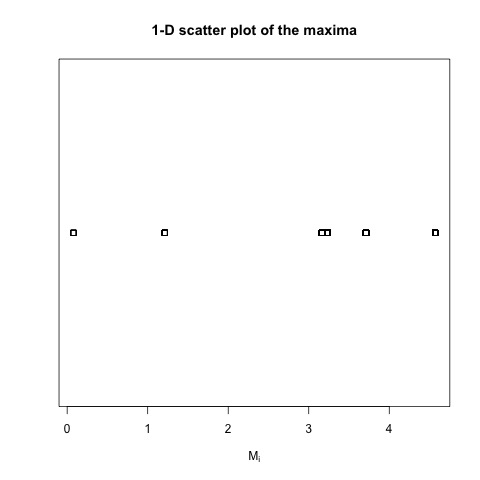
\includegraphics[scale =0.4]{/Users/kimartin/Desktop/PDM_thesis_report/latex_template5_57/main/R_Files_1/gaussianScatterMaxima.jpeg}
        \caption{Scatter Plot of the \\Maxima, n = 10000}
        \label{fig:toyingLimitGaussianScatter}
	\end{minipage}
	\begin{minipage}[b]{0.4\textwidth}
		        \centering
		        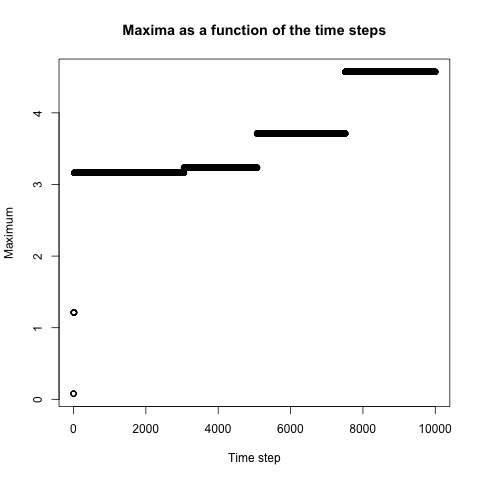
\includegraphics[scale = 0.4]{/Users/kimartin/Desktop/PDM_thesis_report/latex_template5_57/main/R_Files_1/gaussianMaximaAgainstSteps.jpeg}
		        \caption{Maxima against the time steps}
		        \label{fig:toyingLimitGaussianAgainst}
	\end{minipage}
 \end{figure}
 \begin{figure}[h!]
       \centering
       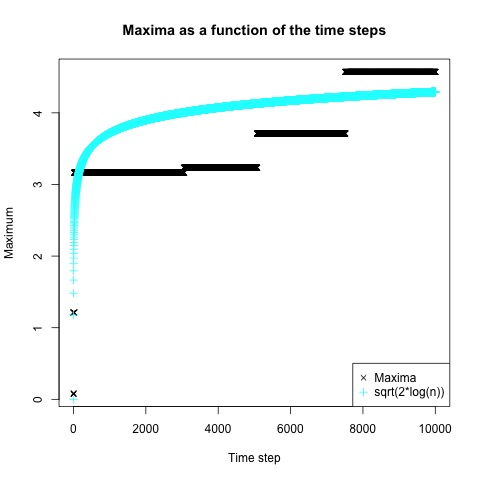
\includegraphics[scale = 0.4]{/Users/kimartin/Desktop/PDM_thesis_report/latex_template5_57/main/R_Files_1/gaussianFitting.jpeg}
       \caption{Maxima against the time steps and function $n \rightarrow \sqrt{2 \log(n)}$}
       \label{fig:toyingLimitGaussianFitting}
\end{figure}
 \begin{figure}[h!]
 	\centering
 	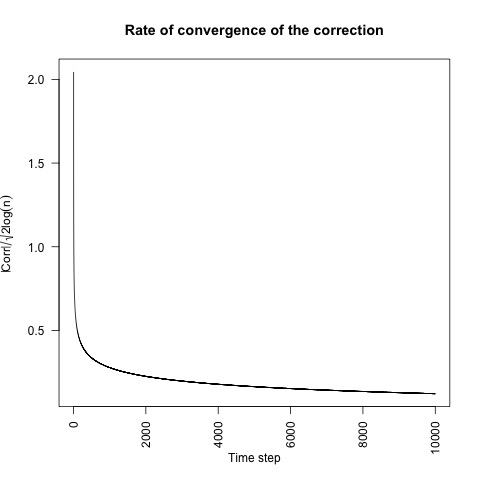
\includegraphics[scale = 0.4]{/Users/kimartin/Desktop/PDM_thesis_report/latex_template5_57/main/R_Files_3/corrApproxQuantileGaussian.jpeg}
 	\caption{The correction becomes negligible compared to the starting term as n grows large}
 	\label{fig:toyingLimitGaussianCorr}
 \end{figure}
\section{Sample following a Cauchy distribution}
\paragraph{Computing the quantiles}
\newline
Let $X_1, \cdots, X_n $ be i.i.d. RVs $\sim$ \textit{Cauchy(0,1)}. The distribution function is $F_X(t) = \frac{1}{\pi} \arctan(x) - \frac{1}{2}$. The $1 - \frac{1}{n}$-quantiles satisfy the equation : 
\newline
\begin{equation}
\begin{alignat*}{2}
&\textcolor{white}{\iff} & F_X(q_n) &= 1 - \frac{1}{n} \\ 
&\iff &  \frac{\arctan(q_n)}{\pi} + \frac{1}{2} &= 1 - \frac{1}{n} \\
&\iff & \frac{\arctan(q_n)}{\pi} &= \frac{2-n}{n} \\
&\iff & q_n &= \tan(\frac{\pi}{2} \frac{2-n}{n})
\end{alignat*}
\end{equation}
\begin{figure}[h!]
		\caption{Below, a realisation of the sequence of maxima for i.i.d. \textit{Cauchy(0,1)} RVs}\label{fig:toyingLimitCauchy}
\end{figure}
\begin{figure}[h!]
	\centering
	\begin{minipage}[b]{0.4\textwidth}
		\centering
		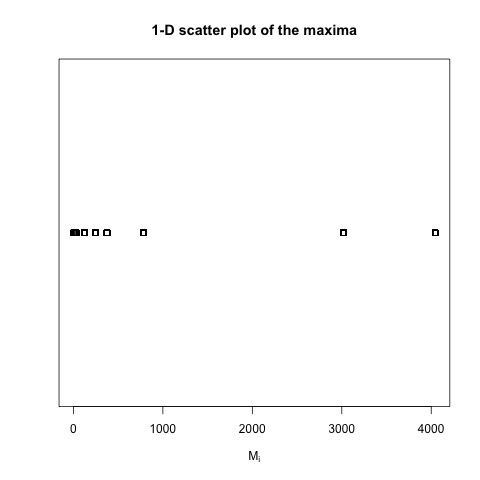
\includegraphics[scale =0.4]{/Users/kimartin/Desktop/PDM_thesis_report/latex_template5_57/main/R_Files_1/cauchyScatterMaxima.jpeg}
		\caption{Scatter Plot of the \\Maxima, n = 10000}
		\label{fig:toyingLimitCauchyScatter}
	\end{minipage}
	\begin{minipage}[b]{0.4\textwidth}
		\centering
		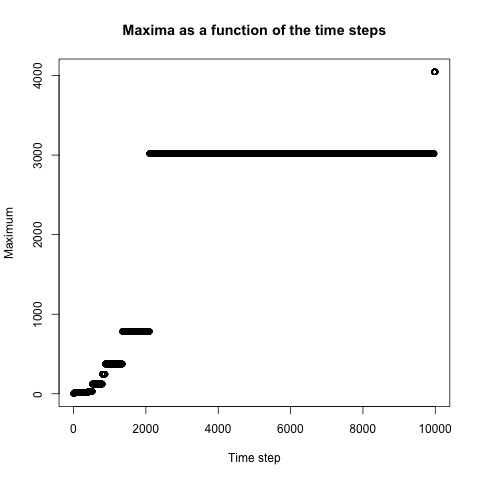
\includegraphics[scale = 0.4]{/Users/kimartin/Desktop/PDM_thesis_report/latex_template5_57/main/R_Files_1/cauchyMaximaAgainstSteps.jpeg}
		\caption{Maxima against the time steps}
		\label{fig:toyingLimitCauchyAgainst}
	\end{minipage}
\end{figure}
 \begin{figure}[h!]
 	\centering
 	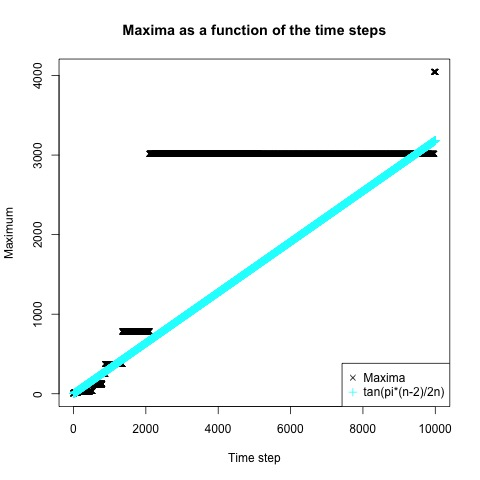
\includegraphics[scale = 0.4]{/Users/kimartin/Desktop/PDM_thesis_report/latex_template5_57/main/R_Files_1/cauchyFitting.jpeg}
    \caption{Maxima against the time steps and function $n \rightarrow \tan(\pi \frac{2-n}{2 n})}$}
    \label{fig:toyingLimitCauchyFitting}
 \end{figure}
\newpage
 \paragraph{}
$n \rightarrow \tan(\pi \frac{2-n}{2 n})}$ is roughly linear in $n$. We know that if $\lvert x \rvert < \frac{\pi}{2}$, $\tan(x) = x + \frac{x^3}{3} + \frac{2 x^5}{15} + \cdots$ so if we take the first order approximation, we get $\tan(x) \approx x$ which confirms what the plot seems to suggest.\footnote{Of course the expansion is valid as for a number of observations $n$ greater than $1$, $ -1 < \frac{2}{n} - 1 < 1$ and thus $\lvert \frac{\pi}{2} \frac{2 - n}{n} \rvert = \vert \frac{\pi}{2} (\frac{2}{n} - 1) \rvert < \frac{\pi}{2}$.}
\section{Sample following an Exponential Distribution}
\paragraph{Computing the quantiles}
\newline
Let $X_1, \cdots, X_n $ be i.i.d. RVs $\sim$ \textit{Exponential($\lambda$)}. The distribution function is $F_X(t) = 1 - \exp(-\lambda t)$. The $1 - \frac{1}{n}$-quantiles satisfy the equation : 
\newline
\begin{equation}
\begin{alignat*}{2}
&\textcolor{white}{\iff} & F_X(q_n) &= 1 - \frac{1}{n} \\ 
&\iff & 1 - \exp(-\lambda q_n) &= 1 - \frac{1}{n} \\
&\iff & q_n &= \frac{1}{\lambda} \log(n)
\end{alignat*}
\end{equation}
\begin{figure}[h!]
		\caption{Below, a realisation of the sequence of maxima for i.i.d. \textit{Exp(1)} RVs}\label{fig:toyingLimitExponential}
\end{figure}
\begin{figure}[h!]
	\centering
	\begin{minipage}[b]{0.4\textwidth}
		\centering
		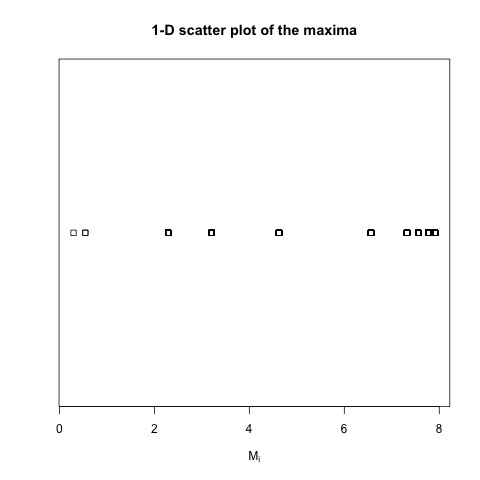
\includegraphics[scale =0.4]{/Users/kimartin/Desktop/PDM_thesis_report/latex_template5_57/main/R_Files_1/exponentialScatterMaxima.jpeg}
		\caption{Scatter Plot of the Maxima, n = 10000}
		\label{fig:toyingLimitExponentialScatter}
	\end{minipage}
	\begin{minipage}[b]{0.4\textwidth}
		\centering
		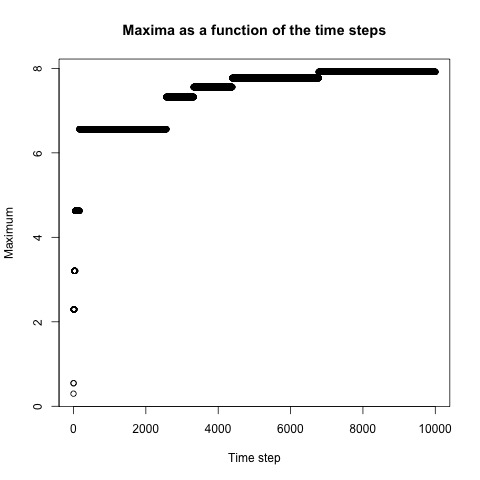
\includegraphics[scale = 0.4]{/Users/kimartin/Desktop/PDM_thesis_report/latex_template5_57/main/R_Files_1/exponentialMaximaAgainstSteps.jpeg}
		\caption{Maxima against the time steps}
		\label{fig:toyingLimitExponentialAgainst}
	\end{minipage}
\end{figure}
\begin{figure}[h!]
		\centering
		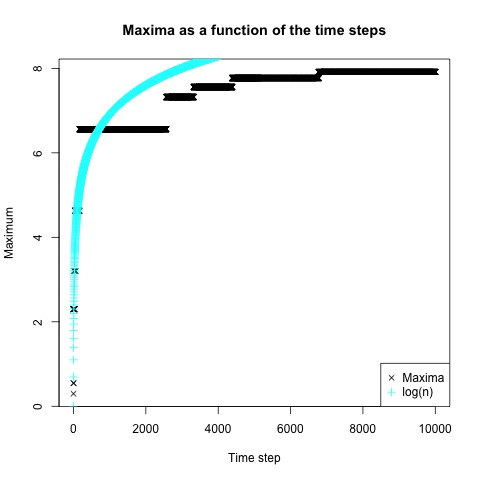
\includegraphics[scale = 0.4]{/Users/kimartin/Desktop/PDM_thesis_report/latex_template5_57/main/R_Files_1/exponentialFitting.jpeg}
		\caption{Maxima against the time steps and function $n \rightarrow \log(n)}$}
	\label{fig:toyingLimitExponentialFitting}
\end{figure}
\newpage
\section{Why does this work ?}
\paragraph{(The underlying idea)}
Why have we made a link between the $\frac{1}{n}$-quantiles of the common distribution of the $X_i$ and the sequence of the $M_n$ ? Actually, the link is that if the sample is made up of independent realizations, then $M_n$ is an estimate of the $1 - \frac{1}{n}$ quantile. \newline
The idea behind this is as follows, that the maxima will get closer to the upper end-point of the distribution of the $X_i$, $F_{X_i}$. That is also the case for the $1 - \frac{1}{n}$-quantiles of $F_{X_i}$. Of course, it is only an intuition !
\section{What are the limiting distributions in theses cases ?}
\paragraph{Preliminary remark}
In what follows we are using theoretical results exposed in the next chapter, chapter 3, concerning the three possible limiting distributions as well as Von Mises' theorem.
\paragraph{Fr\'{e}chet limiting distribution}
Let us assume that a random variable $X$ follows a $Cauchy(0,1)$ distribution, $x^+ = + \infty$. The limiting distribution can only be either a Gumbel or a Fréchet-type distribution.
\begin{equation}
\begin{alignat*}{2}
f_X(x) = \frac{1}{\pi} \frac{1}{1 + x^2}
\end{alignat*}
\end{equation}
\begin{equation}
\begin{alignat*}{2}
F_X(x) = \frac{1}{\pi} \arctan(x) + \frac{1}{2}
\end{alignat*}
\end{equation}
\begin{equation}
\begin{alignat*}{2}
r(x) &= \frac{f_X(x)}{1 - F_X(x)} \\
&= \frac{\frac{1}{1 + x^2}}{\frac{\pi}{2} - \arctan(x)} \\
&= \frac{\frac{1}{1 + x^2}}{\frac{\pi}{2} - (\frac{\pi}{2} - \arctan(\frac{1}{x}))}\\
&= \frac{1}{(1 + x^2) \arctan(\frac{1}{x})}\\
&= \frac{1}{(1 + x^2) (\frac{1}{x} + o(\frac{1}{x^2}))}\\
&= \frac{1}{\frac{1 + x^2}{x} + o(1)}\\
\implies x r(x) &= \frac{x^2}{x^2 + 1 + o(1)} \\
\implies x r(x) &\xrightarrow[x \rightarrow + \infty]{} 1
\end{alignat*}
\end{equation}
Finally, by Von Mises' theorem, we can conclude that the limiting distribution for the standardized maxima of a $Cauchy(0,1)$ sample is a Fréchet distribution.
%\paragraph{Fréchet distribution} 
%Let $X_1, \cdots, X_n $ be i.i.d. RVs $\sim$ \textit{Exponential($\lambda$)}. Let us remember from the previous section the form of the $\frac{1}{n}$-quantile $q_n = \frac{1}{\lambda}\log(n)$. Let us evaluate $F_{M_n}$ in $q_\frac{1}{n}-t$ : \\
%\begin{equation}
%\begin{alignat*}{2}
%F_{M_n}(q_\frac{1}{n}-t) &= (1 - \exp(-\lambda(q_\frac{1}{n}-t)))^n\\ 
%&= (1 - \exp(\lambda t)\exp(-\lambda q_\frac{1}{n}))^n\\ 
%&= (1 - \frac{\exp(\lambda t)}{n})^n \\
%&\longrightarrow_{n \rightarrow +\infty} \exp(-\exp(\lambda t)) \\
%\end{alignat*}
%\end{equation}
\paragraph{Fréchet distribution}
Let us assume that a random variable $X$ follows a $Exp(1)$ distribution, $x^+ = + \infty$. The limiting distribution here again can only be either a Gumbel or a Fréchet-type distribution.
\begin{equation}
\begin{alignat*}{2}
f_X(x) = \lambda \exp(- \lambda x)
\end{alignat*}
\end{equation}
\begin{equation}
\begin{alignat*}{2}
F_X(x) =  1 - \exp(- \lambda x)
\end{alignat*}
\end{equation}
\begin{equation}
\begin{alignat*}{2}
r(x) &= \frac{f_X(x)}{1 - F_X(x)} \\
&= \frac{\lambda \exp(- \lambda x)}{1 - (1 - \exp(- \lambda x))} \\
&= \frac{\lambda \exp(- \lambda x)}{\exp(- \lambda x)} \\
&= \lambda \\
\implies \frac{\mathrm{d}r}{\mathrm{d}x}(x) &= 0
\end{alignat*}
\end{equation}
Finally, by Von Mises' theorem, we can conclude that the limiting distribution for the standardized maxima of an $Exp(1)$ sample is a Gumbel distribution.
\paragraph{Gumbel distribution - bis}
Let us assume that a random variable $X$ follows a $\mathcal{N}(0,1)$ distribution, $x^+ = + \infty$. The limiting distribution here again can only be either a Gumbel or a Fréchet-type distribution. It turns out that in that case, the limiting distribution is a Gumbel-type distribution. The computation is simple, as shown below :
\end{equation}
\begin{equation}
\begin{alignat*}{2}
\frac{\mathrm{d}r}{\mathrm{d}x}(x) &= \frac{\frac{\mathrm{d}f}{\mathrm{d}x}(x) (1 - F_X(x)) - f(x) (-f(x))}{(1 - F_X(x))^2} \\
&= \frac{f(x)^2 + \frac{\mathrm{d}f}{\mathrm{d}x}(x) (1 - F_X(x)) }{(1 - F_X(x))^2}
\end{alignat*}
\end{equation}
It yields an indeterminate form. The key to solve the issue here is to use an expansion of the cumulative distribution function of a standard Gaussian random variable : \newline
$\Phi(x) \approx \frac{1}{2} + \frac{1}{\sqrt{2 \pi}} \exp(\frac{-x^2}{2}) (x + \frac{x^3}{3} + \frac{x^5}{15})$ \newline
\begin{equation}
\begin{alignat*}{2}
\frac{\mathrm{d}r}{\mathrm{d}x}(x) &= \frac{
	\frac{\exp(- x^2)}{2 \pi} - \frac{x}{2 \sqrt{2 \pi}} \exp(\frac{-x^2}{2}) + \frac{x \exp(- x^2)}{2 \pi} (x + \frac{x^3}{3} + \frac{x^5}{15})
	}{
	(\frac{1}{2} - \frac{1}{\sqrt{2 \pi}} \exp(\frac{-x^2}{2}) (x + \frac{x^3}{3} + \frac{x^5}{15}))^2
	} \\
	&=  \frac{
		\frac{\exp(- x^2)}{2 \pi} - \frac{x}{2 \sqrt{2 \pi}} \exp(\frac{-x^2}{2}) + \frac{x \exp(- x^2)}{2 \pi} (x + \frac{x^3}{3} + \frac{x^5}{15})
	}{
	\frac{1}{4} - \frac{\exp(\frac{-x^2}{2})}{\sqrt{2 \pi}} (x + \frac{x^3}{3} + \frac{x^5}{15}) + \frac{\exp(-x^2)}{2 \pi} (x + \frac{x^3}{3} + \frac{x^5}{15})^2 
} \\
\end{alignat*}
\end{equation}
Now we can see that if we take the limit when $x$ goes to $+ \infty$, we get a $0$. By Von Mises' theorem, we can conclude that the limiting distribution for the standardized maxima of a $\mathcal{N}(0,1)$ sample is a Gumbel distribution.
\paragraph{Weibull distribution}
Cauchy, Normal and Exponential distributions all have an infinite upper end-point, thus we will never get a Weibull distribution as limiting distribution. Let us assume that a random variable $X$ follows a $Unif([0,1])$ distribution, $x^+ = 1 < + \infty$. 
\begin{equation}
\begin{alignat*}{2}
f_X(x) = 1
\end{alignat*}
\end{equation}
\begin{equation}
\begin{alignat*}{2}
F_X(x) =  x
\end{alignat*}
\end{equation}
\begin{equation}
\begin{alignat*}{2}
r(x) &= \frac{f_X(x)}{1 - F_X(x)} \\
&= \frac{1}{1 - x} \\
\implies (x^+ - x) r(x) &= (x^+ - x) \frac{1}{1 - x} \\
\implies (1 - x) r(x) &= (1 - x) \frac{1}{1 - x} = 1 \\
\implies (x^+ - x) r(x) &\xrightarrow[x \rightarrow x^+]{} 1 > 0
\end{alignat*}
\end{equation}
Finally, by Von Mises' theorem, we can conclude that the limiting distribution for the standardized maxima of a $Unif([0,1])$ sample is a Weibull distribution.